% Options for packages loaded elsewhere
\PassOptionsToPackage{unicode}{hyperref}
\PassOptionsToPackage{hyphens}{url}
%
\documentclass[
]{article}
\usepackage{amsmath,amssymb}
\usepackage{iftex}
\ifPDFTeX
  \usepackage[T1]{fontenc}
  \usepackage[utf8]{inputenc}
  \usepackage{textcomp} % provide euro and other symbols
\else % if luatex or xetex
  \usepackage{unicode-math} % this also loads fontspec
  \defaultfontfeatures{Scale=MatchLowercase}
  \defaultfontfeatures[\rmfamily]{Ligatures=TeX,Scale=1}
\fi
\usepackage{lmodern}
\ifPDFTeX\else
  % xetex/luatex font selection
\fi
% Use upquote if available, for straight quotes in verbatim environments
\IfFileExists{upquote.sty}{\usepackage{upquote}}{}
\IfFileExists{microtype.sty}{% use microtype if available
  \usepackage[]{microtype}
  \UseMicrotypeSet[protrusion]{basicmath} % disable protrusion for tt fonts
}{}
\makeatletter
\@ifundefined{KOMAClassName}{% if non-KOMA class
  \IfFileExists{parskip.sty}{%
    \usepackage{parskip}
  }{% else
    \setlength{\parindent}{0pt}
    \setlength{\parskip}{6pt plus 2pt minus 1pt}}
}{% if KOMA class
  \KOMAoptions{parskip=half}}
\makeatother
\usepackage{xcolor}
\usepackage[margin=1in]{geometry}
\usepackage{color}
\usepackage{fancyvrb}
\newcommand{\VerbBar}{|}
\newcommand{\VERB}{\Verb[commandchars=\\\{\}]}
\DefineVerbatimEnvironment{Highlighting}{Verbatim}{commandchars=\\\{\}}
% Add ',fontsize=\small' for more characters per line
\usepackage{framed}
\definecolor{shadecolor}{RGB}{248,248,248}
\newenvironment{Shaded}{\begin{snugshade}}{\end{snugshade}}
\newcommand{\AlertTok}[1]{\textcolor[rgb]{0.94,0.16,0.16}{#1}}
\newcommand{\AnnotationTok}[1]{\textcolor[rgb]{0.56,0.35,0.01}{\textbf{\textit{#1}}}}
\newcommand{\AttributeTok}[1]{\textcolor[rgb]{0.13,0.29,0.53}{#1}}
\newcommand{\BaseNTok}[1]{\textcolor[rgb]{0.00,0.00,0.81}{#1}}
\newcommand{\BuiltInTok}[1]{#1}
\newcommand{\CharTok}[1]{\textcolor[rgb]{0.31,0.60,0.02}{#1}}
\newcommand{\CommentTok}[1]{\textcolor[rgb]{0.56,0.35,0.01}{\textit{#1}}}
\newcommand{\CommentVarTok}[1]{\textcolor[rgb]{0.56,0.35,0.01}{\textbf{\textit{#1}}}}
\newcommand{\ConstantTok}[1]{\textcolor[rgb]{0.56,0.35,0.01}{#1}}
\newcommand{\ControlFlowTok}[1]{\textcolor[rgb]{0.13,0.29,0.53}{\textbf{#1}}}
\newcommand{\DataTypeTok}[1]{\textcolor[rgb]{0.13,0.29,0.53}{#1}}
\newcommand{\DecValTok}[1]{\textcolor[rgb]{0.00,0.00,0.81}{#1}}
\newcommand{\DocumentationTok}[1]{\textcolor[rgb]{0.56,0.35,0.01}{\textbf{\textit{#1}}}}
\newcommand{\ErrorTok}[1]{\textcolor[rgb]{0.64,0.00,0.00}{\textbf{#1}}}
\newcommand{\ExtensionTok}[1]{#1}
\newcommand{\FloatTok}[1]{\textcolor[rgb]{0.00,0.00,0.81}{#1}}
\newcommand{\FunctionTok}[1]{\textcolor[rgb]{0.13,0.29,0.53}{\textbf{#1}}}
\newcommand{\ImportTok}[1]{#1}
\newcommand{\InformationTok}[1]{\textcolor[rgb]{0.56,0.35,0.01}{\textbf{\textit{#1}}}}
\newcommand{\KeywordTok}[1]{\textcolor[rgb]{0.13,0.29,0.53}{\textbf{#1}}}
\newcommand{\NormalTok}[1]{#1}
\newcommand{\OperatorTok}[1]{\textcolor[rgb]{0.81,0.36,0.00}{\textbf{#1}}}
\newcommand{\OtherTok}[1]{\textcolor[rgb]{0.56,0.35,0.01}{#1}}
\newcommand{\PreprocessorTok}[1]{\textcolor[rgb]{0.56,0.35,0.01}{\textit{#1}}}
\newcommand{\RegionMarkerTok}[1]{#1}
\newcommand{\SpecialCharTok}[1]{\textcolor[rgb]{0.81,0.36,0.00}{\textbf{#1}}}
\newcommand{\SpecialStringTok}[1]{\textcolor[rgb]{0.31,0.60,0.02}{#1}}
\newcommand{\StringTok}[1]{\textcolor[rgb]{0.31,0.60,0.02}{#1}}
\newcommand{\VariableTok}[1]{\textcolor[rgb]{0.00,0.00,0.00}{#1}}
\newcommand{\VerbatimStringTok}[1]{\textcolor[rgb]{0.31,0.60,0.02}{#1}}
\newcommand{\WarningTok}[1]{\textcolor[rgb]{0.56,0.35,0.01}{\textbf{\textit{#1}}}}
\usepackage{graphicx}
\makeatletter
\newsavebox\pandoc@box
\newcommand*\pandocbounded[1]{% scales image to fit in text height/width
  \sbox\pandoc@box{#1}%
  \Gscale@div\@tempa{\textheight}{\dimexpr\ht\pandoc@box+\dp\pandoc@box\relax}%
  \Gscale@div\@tempb{\linewidth}{\wd\pandoc@box}%
  \ifdim\@tempb\p@<\@tempa\p@\let\@tempa\@tempb\fi% select the smaller of both
  \ifdim\@tempa\p@<\p@\scalebox{\@tempa}{\usebox\pandoc@box}%
  \else\usebox{\pandoc@box}%
  \fi%
}
% Set default figure placement to htbp
\def\fps@figure{htbp}
\makeatother
\setlength{\emergencystretch}{3em} % prevent overfull lines
\providecommand{\tightlist}{%
  \setlength{\itemsep}{0pt}\setlength{\parskip}{0pt}}
\setcounter{secnumdepth}{-\maxdimen} % remove section numbering
\usepackage{ctex}
\usepackage{bookmark}
\IfFileExists{xurl.sty}{\usepackage{xurl}}{} % add URL line breaks if available
\urlstyle{same}
\hypersetup{
  pdftitle={finaltest},
  pdfauthor={zza},
  hidelinks,
  pdfcreator={LaTeX via pandoc}}

\title{finaltest}
\author{zza}
\date{2025-07-02}

\begin{document}
\maketitle

\subsection{1}\label{section}

\begin{Shaded}
\begin{Highlighting}[]
\NormalTok{matrix }\OtherTok{\textless{}{-}} \FunctionTok{matrix}\NormalTok{(}\FunctionTok{c}\NormalTok{(}\DecValTok{9}\NormalTok{, }\DecValTok{4}\NormalTok{, }\DecValTok{12}\NormalTok{, }\DecValTok{2}\NormalTok{,}
                   \DecValTok{5}\NormalTok{, }\DecValTok{0}\NormalTok{, }\DecValTok{7}\NormalTok{, }\DecValTok{9}\NormalTok{,}
                   \DecValTok{2}\NormalTok{, }\DecValTok{6}\NormalTok{, }\DecValTok{8}\NormalTok{, }\DecValTok{0}\NormalTok{,}
                   \DecValTok{9}\NormalTok{, }\DecValTok{2}\NormalTok{, }\DecValTok{9}\NormalTok{, }\DecValTok{11}\NormalTok{), }
                 \AttributeTok{nrow =} \DecValTok{4}\NormalTok{, }\AttributeTok{byrow =} \ConstantTok{TRUE}\NormalTok{)}


\NormalTok{inverse\_matrix }\OtherTok{\textless{}{-}} \FunctionTok{solve}\NormalTok{(matrix)}


\NormalTok{verification }\OtherTok{\textless{}{-}}\NormalTok{ matrix }\SpecialCharTok{\%*\%}\NormalTok{ inverse\_matrix}
\FunctionTok{all.equal}\NormalTok{(verification, }\FunctionTok{diag}\NormalTok{(}\DecValTok{4}\NormalTok{))}
\end{Highlighting}
\end{Shaded}

\begin{verbatim}
## [1] TRUE
\end{verbatim}

\subsection{2}\label{section-1}

\subsubsection{a}\label{a}

\begin{Shaded}
\begin{Highlighting}[]
\NormalTok{xVec }\OtherTok{\textless{}{-}} \FunctionTok{sample}\NormalTok{(}\DecValTok{0}\SpecialCharTok{:}\DecValTok{999}\NormalTok{, }\DecValTok{250}\NormalTok{, }\AttributeTok{replace=}\NormalTok{T)}
\NormalTok{yVec }\OtherTok{\textless{}{-}} \FunctionTok{sample}\NormalTok{(}\DecValTok{0}\SpecialCharTok{:}\DecValTok{999}\NormalTok{, }\DecValTok{250}\NormalTok{, }\AttributeTok{replace=}\NormalTok{T)}

\DocumentationTok{\#\# a}
\NormalTok{newVec }\OtherTok{\textless{}{-}}\NormalTok{ yVec[}\DecValTok{2}\SpecialCharTok{:}\DecValTok{250}\NormalTok{] }\SpecialCharTok{{-}}\NormalTok{ xVec[}\DecValTok{1}\SpecialCharTok{:}\DecValTok{249}\NormalTok{]}
\NormalTok{newVec}
\end{Highlighting}
\end{Shaded}

\begin{verbatim}
##   [1] -192   48 -755  169  487  285 -296 -422   15  225  363 -335  294   35   -8
##  [16]  395 -730 -465 -583  165  156   98  725  350   54  662 -307   13 -199  397
##  [31]  831  248 -445  723 -534  -43 -415  -53 -465 -793 -722  214   75 -241   50
##  [46] -787  272  245 -374    0 -789 -143  -92  781 -270  154 -539  281  570  -54
##  [61] -686  262 -354  816 -653   -5  415  366  189 -149 -139  381  -63  -45  612
##  [76]  193   -6  332 -587 -710 -238 -110  770 -178  470 -375 -904  -63 -680  109
##  [91] -269  571 -578 -323  178  145 -115   87  435  409  323  467  161  290  350
## [106] -190  -69  228  231 -791 -532 -268 -387   -2  522  223  961   44 -112 -124
## [121]  563 -693 -430  743  721  406 -675  492 -778   34   46 -356 -412  581 -747
## [136]  -61  -19   76 -524  512  305  176   52  -56  302 -112 -557  107   41  148
## [151]  569 -116 -521  302 -529 -257  -75  128 -633   31  411  108  213  668 -308
## [166]  395  -92 -496 -429 -446  -93   86   -7  114 -499  199  -11   79 -423 -733
## [181]  686  414  189  969  584  903  -75 -344  902  176 -747 -535  -32 -235  218
## [196]   75 -509  535 -605 -571 -830  -47  425  -24   54 -624  340  -13  526 -140
## [211] -803  798  123 -525 -349   44  -50 -711  631   36  268  615 -329  240  368
## [226]  913 -331  422 -319  849 -180 -211 -184  751 -285  459 -110  149 -514  -96
## [241]  -35 -541  178  -15 -241 -754  142 -179  200
\end{verbatim}

\subsubsection{b}\label{b}

\begin{Shaded}
\begin{Highlighting}[]
\NormalTok{values\_greater\_600 }\OtherTok{\textless{}{-}}\NormalTok{ yVec[yVec }\SpecialCharTok{\textgreater{}} \DecValTok{600}\NormalTok{]}
\NormalTok{values\_greater\_600}
\end{Highlighting}
\end{Shaded}

\begin{verbatim}
##  [1] 714 988 927 885 722 909 610 914 882 903 754 838 874 761 692 680 870 958 663
## [20] 912 929 904 828 999 800 908 997 973 989 960 767 645 996 606 853 681 801 977
## [39] 737 837 709 755 867 824 765 622 975 810 923 794 713 718 909 910 827 813 683
## [58] 857 899 638 853 916 749 982 935 933 664 970 762 980 971 788 964 885 745 808
## [77] 942 642 830 873 854 757 690 929 981 788 614 940
\end{verbatim}

\subsubsection{c}\label{c}

\begin{Shaded}
\begin{Highlighting}[]
\NormalTok{indices\_greater\_600 }\OtherTok{\textless{}{-}} \FunctionTok{which}\NormalTok{(yVec }\SpecialCharTok{\textgreater{}} \DecValTok{600}\NormalTok{)}
\NormalTok{indices\_greater\_600}
\end{Highlighting}
\end{Shaded}

\begin{verbatim}
##  [1]   2   6  11  14  16  17  22  24  27  29  31  32  33  35  43  44  49  55  60
## [20]  65  67  69  72  73  74  76  77  84  86 100 101 102 103 105 109 110 116 118
## [39] 120 121 122 125 126 132 135 137 139 141 142 145 146 151 152 159 162 165 167
## [58] 168 172 175 177 178 182 185 186 187 188 190 191 199 204 205 208 209 210 211
## [77] 213 218 220 221 223 225 226 227 231 235 237 250
\end{verbatim}

\subsubsection{d}\label{d}

\begin{Shaded}
\begin{Highlighting}[]
\NormalTok{sorted\_xVec }\OtherTok{\textless{}{-}}\NormalTok{ xVec[}\FunctionTok{order}\NormalTok{(yVec)]}
\NormalTok{sorted\_xVec}
\end{Highlighting}
\end{Shaded}

\begin{verbatim}
##   [1] 626 380 571  72 478  90 199 625 506 209 191 357 793 884 222 524 778  30
##  [19] 622 554 849 288  19 596 606 739 176  41 970 485  50 877 184  12 416 125
##  [37] 683 144  38 278 325 228 782  63 277 191 216 890 263 373 975 284 734 888
##  [55] 811 759 501  93 155 741 570 592  68 989 568 888   5  37 184 869 752 947
##  [73] 675 777 149 699 591 624 279 546  13   9 654 523 525 692 510  82 934 372
##  [91] 303 298 220 681  96 850 909 517 280 230 702  16 483 145 433 203 531 762
## [109] 984 992 101 445  34 441 454 737 127 939 704 298 538 906 899 246 177 524
## [127] 519 930 289 730 736 880 450 132 958 316 480 816 652 797 525  97 264 944
## [145] 239 535 610 967 625  93 899 189 848 296 726 686 272 694 984 520 740 579
## [163] 226 464 438 490 797 728 529 491 572 737 896 949  16 605 767 630 207 340
## [181] 514 961 948  24   7 146 322 836 868 875 322 507 498 411 620 168 934 618
## [199] 399 904  48 618 837 146 626 450 927 693 996 172 494 275 579 469 458 219
## [217] 311 242 277 804 741 708 844 983 133  26 166 191  55 347 739  30 606 311
## [235] 310 358 898 586 812 656 991  31 821 253 351 311 840 339  42 863
\end{verbatim}

\subsubsection{e}\label{e}

\begin{Shaded}
\begin{Highlighting}[]
\NormalTok{selected\_elements }\OtherTok{\textless{}{-}}\NormalTok{ yVec[}\FunctionTok{seq}\NormalTok{(}\DecValTok{1}\NormalTok{, }\DecValTok{250}\NormalTok{, }\AttributeTok{by =} \DecValTok{3}\NormalTok{)]}
\NormalTok{selected\_elements}
\end{Highlighting}
\end{Shaded}

\begin{verbatim}
##  [1] 471 114 596 388 275 722 106 610 483 162 754 134 480 114 692 500 870   4 958
## [20] 142 437 345 929 466 999 908 541 521 478  35 331 116 586 960 996 576 853  64
## [39] 278 977 837 124 578  70 548 128 975 923 794 240 718 463 369 211 156  91 500
## [58] 899 638 916 155 290 933 970 342 252 980 145 788 964 808 434 308 830 854 690
## [77] 512  73 788 328 150 327 126 940
\end{verbatim}

\subsection{3}\label{section-2}

\subsubsection{a}\label{a-1}

\begin{Shaded}
\begin{Highlighting}[]
\FunctionTok{data}\NormalTok{(state) }
\NormalTok{state.x77 }\OtherTok{\textless{}{-}} \FunctionTok{as\_tibble}\NormalTok{(state.x77, }\AttributeTok{rownames =} \StringTok{\textquotesingle{}State\textquotesingle{}}\NormalTok{)}

\NormalTok{low\_income\_states }\OtherTok{\textless{}{-}}\NormalTok{ state.x77 }\SpecialCharTok{\%\textgreater{}\%} \FunctionTok{filter}\NormalTok{(Income }\SpecialCharTok{\textless{}} \DecValTok{4300}\NormalTok{)}
\NormalTok{avg\_income\_low }\OtherTok{\textless{}{-}} \FunctionTok{mean}\NormalTok{(low\_income\_states}\SpecialCharTok{$}\NormalTok{Income)}
\FunctionTok{cat}\NormalTok{(}\StringTok{"收入低于4300的州的平均收入:"}\NormalTok{, avg\_income\_low)}
\end{Highlighting}
\end{Shaded}

\begin{verbatim}
## 收入低于4300的州的平均收入: 3830.6
\end{verbatim}

\subsubsection{b}\label{b-1}

\begin{Shaded}
\begin{Highlighting}[]
\NormalTok{highest\_income\_state }\OtherTok{\textless{}{-}}\NormalTok{ state.x77 }\SpecialCharTok{\%\textgreater{}\%} 
  \FunctionTok{arrange}\NormalTok{(}\FunctionTok{desc}\NormalTok{(Income)) }\SpecialCharTok{\%\textgreater{}\%} 
  \FunctionTok{slice}\NormalTok{(}\DecValTok{1}\NormalTok{) }\SpecialCharTok{\%\textgreater{}\%} 
  \FunctionTok{pull}\NormalTok{(State)}
\FunctionTok{cat}\NormalTok{(}\StringTok{"收入最高的州:"}\NormalTok{, highest\_income\_state)}
\end{Highlighting}
\end{Shaded}

\begin{verbatim}
## 收入最高的州: Alaska
\end{verbatim}

\subsubsection{c}\label{c-1}

\begin{Shaded}
\begin{Highlighting}[]
\NormalTok{state.x77 }\OtherTok{\textless{}{-}}\NormalTok{ state.x77 }\SpecialCharTok{\%\textgreater{}\%} 
  \FunctionTok{mutate}\NormalTok{(}\AttributeTok{Population\_size =} \FunctionTok{ifelse}\NormalTok{(Population }\SpecialCharTok{\textless{}=} \DecValTok{4500}\NormalTok{, }\StringTok{"S"}\NormalTok{, }\StringTok{"L"}\NormalTok{))}
\end{Highlighting}
\end{Shaded}

\subsubsection{d}\label{d-1}

\begin{Shaded}
\begin{Highlighting}[]
\NormalTok{grouped\_stats }\OtherTok{\textless{}{-}}\NormalTok{ state.x77 }\SpecialCharTok{\%\textgreater{}\%} 
  \FunctionTok{group\_by}\NormalTok{(Population\_size) }\SpecialCharTok{\%\textgreater{}\%} 
  \FunctionTok{summarize}\NormalTok{(}\AttributeTok{avg\_income =} \FunctionTok{mean}\NormalTok{(Income), }\AttributeTok{avg\_illiteracy =} \FunctionTok{mean}\NormalTok{(Illiteracy))}
\NormalTok{grouped\_stats}
\end{Highlighting}
\end{Shaded}

\begin{verbatim}
## # A tibble: 2 x 3
##   Population_size avg_income avg_illiteracy
##   <chr>                <dbl>          <dbl>
## 1 L                    4608.           1.2 
## 2 S                    4355.           1.16
\end{verbatim}

\subsection{4}\label{section-3}

\subsubsection{a}\label{a-2}

\begin{Shaded}
\begin{Highlighting}[]
\NormalTok{simulate\_uniform }\OtherTok{\textless{}{-}} \ControlFlowTok{function}\NormalTok{(n) \{}

  \FunctionTok{tibble}\NormalTok{(}
    \AttributeTok{X1 =} \FunctionTok{runif}\NormalTok{(n, }\AttributeTok{min =} \DecValTok{0}\NormalTok{, }\AttributeTok{max =} \DecValTok{1}\NormalTok{),}
    \AttributeTok{X2 =} \FunctionTok{runif}\NormalTok{(n, }\AttributeTok{min =} \DecValTok{0}\NormalTok{, }\AttributeTok{max =} \DecValTok{1}\NormalTok{)}
\NormalTok{  )}
\NormalTok{\}}
\end{Highlighting}
\end{Shaded}

\subsubsection{b}\label{b-2}

\begin{Shaded}
\begin{Highlighting}[]
\NormalTok{calculate\_proportions }\OtherTok{\textless{}{-}} \ControlFlowTok{function}\NormalTok{(observations) \{}
  \ControlFlowTok{if}\NormalTok{ (}\SpecialCharTok{!}\FunctionTok{all}\NormalTok{(}\FunctionTok{c}\NormalTok{(}\StringTok{"X1"}\NormalTok{, }\StringTok{"X2"}\NormalTok{) }\SpecialCharTok{\%in\%} \FunctionTok{colnames}\NormalTok{(observations))) \{}
    \FunctionTok{stop}\NormalTok{(}\StringTok{"输入数据必须包含X1和X2列"}\NormalTok{)}
\NormalTok{  \}}
  
\NormalTok{  n }\OtherTok{\textless{}{-}} \FunctionTok{nrow}\NormalTok{(observations)}
  

\NormalTok{  dist\_to\_edges }\OtherTok{\textless{}{-}} \FunctionTok{pmin}\NormalTok{(}
\NormalTok{    observations}\SpecialCharTok{$}\NormalTok{X1,            }
    \DecValTok{1} \SpecialCharTok{{-}}\NormalTok{ observations}\SpecialCharTok{$}\NormalTok{X1,        }
\NormalTok{    observations}\SpecialCharTok{$}\NormalTok{X2,           }
    \DecValTok{1} \SpecialCharTok{{-}}\NormalTok{ observations}\SpecialCharTok{$}\NormalTok{X2         }
\NormalTok{  )}
\NormalTok{  prop\_edges }\OtherTok{\textless{}{-}} \FunctionTok{mean}\NormalTok{(dist\_to\_edges }\SpecialCharTok{\textless{}} \FloatTok{0.25}\NormalTok{)  }
  

\NormalTok{  vertices }\OtherTok{\textless{}{-}} \FunctionTok{matrix}\NormalTok{(}\FunctionTok{c}\NormalTok{(}\DecValTok{0}\NormalTok{, }\DecValTok{0}\NormalTok{, }\DecValTok{0}\NormalTok{, }\DecValTok{1}\NormalTok{, }\DecValTok{1}\NormalTok{, }\DecValTok{0}\NormalTok{, }\DecValTok{1}\NormalTok{, }\DecValTok{1}\NormalTok{), }\AttributeTok{ncol =} \DecValTok{2}\NormalTok{, }\AttributeTok{byrow =} \ConstantTok{TRUE}\NormalTok{)}
  

\NormalTok{  dist\_to\_vertices }\OtherTok{\textless{}{-}} \FunctionTok{apply}\NormalTok{(vertices, }\DecValTok{1}\NormalTok{, }\ControlFlowTok{function}\NormalTok{(vertex) \{}
    \FunctionTok{sqrt}\NormalTok{(}
\NormalTok{      (observations}\SpecialCharTok{$}\NormalTok{X1 }\SpecialCharTok{{-}}\NormalTok{ vertex[}\DecValTok{1}\NormalTok{])}\SpecialCharTok{\^{}}\DecValTok{2} \SpecialCharTok{+} 
\NormalTok{      (observations}\SpecialCharTok{$}\NormalTok{X2 }\SpecialCharTok{{-}}\NormalTok{ vertex[}\DecValTok{2}\NormalTok{])}\SpecialCharTok{\^{}} \DecValTok{2}
\NormalTok{    )}
\NormalTok{  \})}
  

\NormalTok{  min\_dist\_vertices }\OtherTok{\textless{}{-}} \FunctionTok{apply}\NormalTok{(dist\_to\_vertices, }\DecValTok{1}\NormalTok{, min)}
\NormalTok{  prop\_vertices }\OtherTok{\textless{}{-}} \FunctionTok{mean}\NormalTok{(min\_dist\_vertices }\SpecialCharTok{\textless{}} \FloatTok{0.25}\NormalTok{)}
  

  \FunctionTok{return}\NormalTok{(}\FunctionTok{list}\NormalTok{(}
    \AttributeTok{proportion\_edges =}\NormalTok{ prop\_edges,}
    \AttributeTok{proportion\_vertices =}\NormalTok{ prop\_vertices}
\NormalTok{  ))}
\NormalTok{\}}



\DocumentationTok{\#\#验证两个函数}
\FunctionTok{set.seed}\NormalTok{(}\DecValTok{123}\NormalTok{)}
\NormalTok{obs }\OtherTok{\textless{}{-}} \FunctionTok{simulate\_uniform}\NormalTok{(}\DecValTok{10000}\NormalTok{)}

\CommentTok{\# 计算比例}
\NormalTok{results }\OtherTok{\textless{}{-}} \FunctionTok{calculate\_proportions}\NormalTok{(obs)}


\FunctionTok{cat}\NormalTok{(}\StringTok{"到最近边距离\textless{}0.25的比例:"}\NormalTok{, results}\SpecialCharTok{$}\NormalTok{proportion\_edges, }\StringTok{"}\SpecialCharTok{\textbackslash{}n}\StringTok{"}\NormalTok{)}
\end{Highlighting}
\end{Shaded}

\begin{verbatim}
## 到最近边距离<0.25的比例: 0.7493
\end{verbatim}

\begin{Shaded}
\begin{Highlighting}[]
\FunctionTok{cat}\NormalTok{(}\StringTok{"到最近顶点距离\textless{}0.25的比例:"}\NormalTok{, results}\SpecialCharTok{$}\NormalTok{proportion\_vertices)}
\end{Highlighting}
\end{Shaded}

\begin{verbatim}
## 到最近顶点距离<0.25的比例: 0.1948
\end{verbatim}

\subsection{5}\label{section-4}

\subsubsection{a}\label{a-3}

\begin{Shaded}
\begin{Highlighting}[]
\NormalTok{n }\OtherTok{\textless{}{-}} \DecValTok{10000}
\FunctionTok{set.seed}\NormalTok{(}\DecValTok{1}\NormalTok{)}
\NormalTok{points }\OtherTok{\textless{}{-}} \FunctionTok{tibble}\NormalTok{(}\StringTok{"x"} \OtherTok{=} \FunctionTok{runif}\NormalTok{(n), }\StringTok{"y"} \OtherTok{=} \FunctionTok{runif}\NormalTok{(n))}

\NormalTok{points }\OtherTok{\textless{}{-}}\NormalTok{ points }\SpecialCharTok{|\textgreater{}}
\FunctionTok{mutate}\NormalTok{(}\AttributeTok{inside =} \FunctionTok{map2\_dbl}\NormalTok{(}\AttributeTok{.x =}\NormalTok{ x, }\AttributeTok{.y =}\NormalTok{ y, }\SpecialCharTok{\textasciitilde{}}\FunctionTok{ifelse}\NormalTok{(.x}\SpecialCharTok{**}\DecValTok{2} \SpecialCharTok{+}\NormalTok{ .y}\SpecialCharTok{**}\DecValTok{2} \SpecialCharTok{\textless{}} \DecValTok{1}\NormalTok{, }\DecValTok{1}\NormalTok{, }\DecValTok{0}\NormalTok{))) }\SpecialCharTok{|\textgreater{}}
\FunctionTok{rowid\_to\_column}\NormalTok{(}\StringTok{"N"}\NormalTok{)}


\NormalTok{points }\OtherTok{\textless{}{-}}\NormalTok{ points }\SpecialCharTok{|\textgreater{}}
  \FunctionTok{mutate}\NormalTok{(}\AttributeTok{cumulative\_inside =} \FunctionTok{cumsum}\NormalTok{(inside),}
         \AttributeTok{pi\_estimate =} \DecValTok{4} \SpecialCharTok{*}\NormalTok{ cumulative\_inside }\SpecialCharTok{/}\NormalTok{ N)}

\CommentTok{\# 查看后几行的估计值}
\FunctionTok{tail}\NormalTok{(points[, }\FunctionTok{c}\NormalTok{(}\StringTok{"N"}\NormalTok{, }\StringTok{"inside"}\NormalTok{, }\StringTok{"cumulative\_inside"}\NormalTok{, }\StringTok{"pi\_estimate"}\NormalTok{)])}
\end{Highlighting}
\end{Shaded}

\begin{verbatim}
## # A tibble: 6 x 4
##       N inside cumulative_inside pi_estimate
##   <int>  <dbl>             <dbl>       <dbl>
## 1  9995      1              7824        3.13
## 2  9996      0              7824        3.13
## 3  9997      1              7825        3.13
## 4  9998      1              7826        3.13
## 5  9999      1              7827        3.13
## 6 10000      1              7828        3.13
\end{verbatim}

\subsubsection{b}\label{b-3}

\begin{Shaded}
\begin{Highlighting}[]
\FunctionTok{library}\NormalTok{(ggplot2)}
\FunctionTok{ggplot}\NormalTok{(points, }\FunctionTok{aes}\NormalTok{(}\AttributeTok{x =}\NormalTok{ N, }\AttributeTok{y =}\NormalTok{ pi\_estimate)) }\SpecialCharTok{+}
  \FunctionTok{geom\_line}\NormalTok{(}\AttributeTok{color =} \StringTok{"blue"}\NormalTok{) }\SpecialCharTok{+}
  \FunctionTok{geom\_hline}\NormalTok{(}\AttributeTok{yintercept =}\NormalTok{ pi, }\AttributeTok{color =} \StringTok{"red"}\NormalTok{, }\AttributeTok{linetype =} \StringTok{"dashed"}\NormalTok{) }\SpecialCharTok{+}
  \FunctionTok{labs}\NormalTok{(}\AttributeTok{title =} \StringTok{"蒙特卡洛模拟估计π"}\NormalTok{,}
       \AttributeTok{x =} \StringTok{"箭头数量N"}\NormalTok{,}
       \AttributeTok{y =} \StringTok{"π的估计值"}\NormalTok{) }\SpecialCharTok{+}
  \FunctionTok{theme\_minimal}\NormalTok{()}
\end{Highlighting}
\end{Shaded}

\pandocbounded{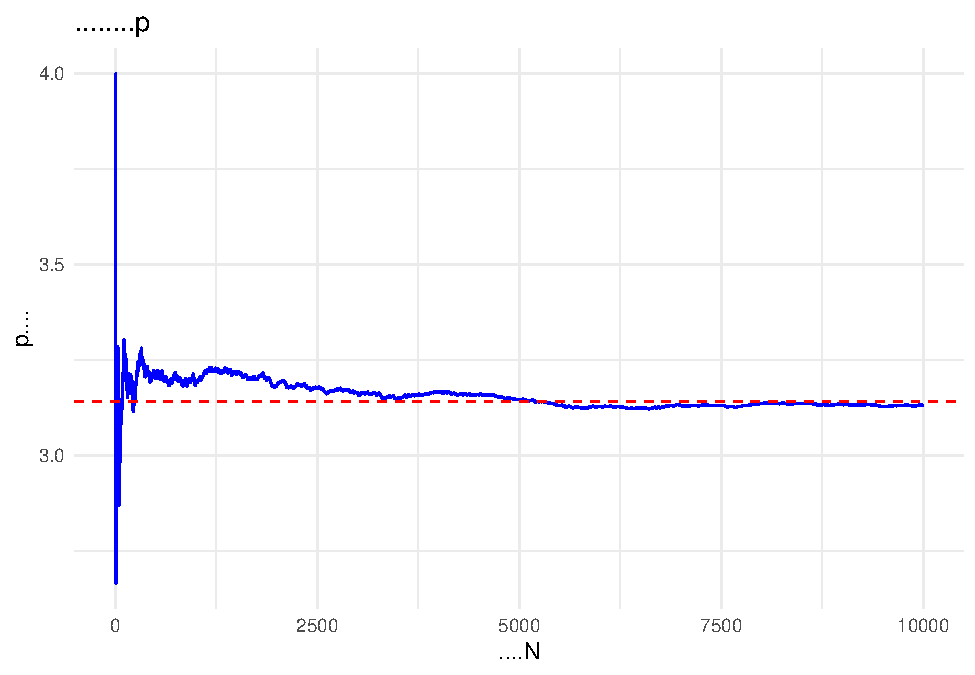
\includegraphics[keepaspectratio]{test_files/figure-latex/unnamed-chunk-15-1.pdf}}

\subsection{6}\label{section-5}

\subsubsection{a}\label{a-4}

\begin{Shaded}
\begin{Highlighting}[]
\NormalTok{suicrates }\OtherTok{\textless{}{-}} \FunctionTok{tibble}\NormalTok{(}
  \AttributeTok{Country =} \FunctionTok{c}\NormalTok{(}\StringTok{\textquotesingle{}Canada\textquotesingle{}}\NormalTok{, }\StringTok{\textquotesingle{}Israel\textquotesingle{}}\NormalTok{, }\StringTok{\textquotesingle{}Japan\textquotesingle{}}\NormalTok{, }\StringTok{\textquotesingle{}Austria\textquotesingle{}}\NormalTok{, }\StringTok{\textquotesingle{}France\textquotesingle{}}\NormalTok{, }\StringTok{\textquotesingle{}Germany\textquotesingle{}}\NormalTok{, }
              \StringTok{\textquotesingle{}Hungary\textquotesingle{}}\NormalTok{, }\StringTok{\textquotesingle{}Italy\textquotesingle{}}\NormalTok{, }\StringTok{\textquotesingle{}Netherlands\textquotesingle{}}\NormalTok{, }\StringTok{\textquotesingle{}Poland\textquotesingle{}}\NormalTok{, }\StringTok{\textquotesingle{}Spain\textquotesingle{}}\NormalTok{, }\StringTok{\textquotesingle{}Sweden\textquotesingle{}}\NormalTok{, }
              \StringTok{\textquotesingle{}Switzerland\textquotesingle{}}\NormalTok{, }\StringTok{\textquotesingle{}UK\textquotesingle{}}\NormalTok{, }\StringTok{\textquotesingle{}USA\textquotesingle{}}\NormalTok{),}
  \AttributeTok{Age25.34 =} \FunctionTok{c}\NormalTok{(}\DecValTok{22}\NormalTok{, }\DecValTok{9}\NormalTok{, }\DecValTok{22}\NormalTok{, }\DecValTok{29}\NormalTok{, }\DecValTok{16}\NormalTok{, }\DecValTok{28}\NormalTok{, }\DecValTok{48}\NormalTok{, }\DecValTok{7}\NormalTok{, }\DecValTok{8}\NormalTok{, }\DecValTok{26}\NormalTok{, }\DecValTok{4}\NormalTok{, }\DecValTok{28}\NormalTok{, }\DecValTok{22}\NormalTok{, }\DecValTok{10}\NormalTok{, }\DecValTok{20}\NormalTok{),}
  \AttributeTok{Age35.44 =} \FunctionTok{c}\NormalTok{(}\DecValTok{27}\NormalTok{, }\DecValTok{19}\NormalTok{, }\DecValTok{19}\NormalTok{, }\DecValTok{40}\NormalTok{, }\DecValTok{25}\NormalTok{, }\DecValTok{35}\NormalTok{, }\DecValTok{65}\NormalTok{, }\DecValTok{8}\NormalTok{, }\DecValTok{11}\NormalTok{, }\DecValTok{29}\NormalTok{, }\DecValTok{7}\NormalTok{, }\DecValTok{41}\NormalTok{, }\DecValTok{34}\NormalTok{, }\DecValTok{13}\NormalTok{, }\DecValTok{22}\NormalTok{),}
  \AttributeTok{Age45.54 =} \FunctionTok{c}\NormalTok{(}\DecValTok{31}\NormalTok{, }\DecValTok{10}\NormalTok{, }\DecValTok{21}\NormalTok{, }\DecValTok{52}\NormalTok{, }\DecValTok{36}\NormalTok{, }\DecValTok{41}\NormalTok{, }\DecValTok{84}\NormalTok{, }\DecValTok{11}\NormalTok{, }\DecValTok{18}\NormalTok{, }\DecValTok{36}\NormalTok{, }\DecValTok{10}\NormalTok{, }\DecValTok{46}\NormalTok{, }\DecValTok{41}\NormalTok{, }\DecValTok{15}\NormalTok{, }\DecValTok{28}\NormalTok{),}
  \AttributeTok{Age55.64 =} \FunctionTok{c}\NormalTok{(}\DecValTok{34}\NormalTok{, }\DecValTok{14}\NormalTok{, }\DecValTok{31}\NormalTok{, }\DecValTok{53}\NormalTok{, }\DecValTok{47}\NormalTok{, }\DecValTok{49}\NormalTok{, }\DecValTok{81}\NormalTok{, }\DecValTok{18}\NormalTok{, }\DecValTok{20}\NormalTok{, }\DecValTok{32}\NormalTok{, }\DecValTok{16}\NormalTok{, }\DecValTok{51}\NormalTok{, }\DecValTok{50}\NormalTok{, }\DecValTok{17}\NormalTok{, }\DecValTok{33}\NormalTok{),}
  \AttributeTok{Age65.74 =} \FunctionTok{c}\NormalTok{(}\DecValTok{24}\NormalTok{, }\DecValTok{27}\NormalTok{, }\DecValTok{49}\NormalTok{, }\DecValTok{69}\NormalTok{, }\DecValTok{56}\NormalTok{, }\DecValTok{52}\NormalTok{, }\DecValTok{107}\NormalTok{, }\DecValTok{27}\NormalTok{, }\DecValTok{28}\NormalTok{, }\DecValTok{28}\NormalTok{, }\DecValTok{22}\NormalTok{, }\DecValTok{35}\NormalTok{, }\DecValTok{51}\NormalTok{, }\DecValTok{22}\NormalTok{, }\DecValTok{37}\NormalTok{)}
\NormalTok{)}


\FunctionTok{library}\NormalTok{(tidyr)}
\NormalTok{suicrates\_long }\OtherTok{\textless{}{-}}\NormalTok{ suicrates }\SpecialCharTok{\%\textgreater{}\%} 
  \FunctionTok{pivot\_longer}\NormalTok{(}\AttributeTok{cols =} \SpecialCharTok{{-}}\NormalTok{Country, }
               \AttributeTok{names\_to =} \StringTok{"AgeGroup"}\NormalTok{, }
               \AttributeTok{values\_to =} \StringTok{"SuicideRate"}\NormalTok{)}
\end{Highlighting}
\end{Shaded}

\subsubsection{b}\label{b-4}

\begin{Shaded}
\begin{Highlighting}[]
\FunctionTok{library}\NormalTok{(ggplot2)}
\FunctionTok{ggplot}\NormalTok{(suicrates\_long, }\FunctionTok{aes}\NormalTok{(}\AttributeTok{x =}\NormalTok{ AgeGroup, }\AttributeTok{y =}\NormalTok{ SuicideRate, }\AttributeTok{fill =}\NormalTok{ AgeGroup)) }\SpecialCharTok{+}
  \FunctionTok{geom\_boxplot}\NormalTok{() }\SpecialCharTok{+}
  \FunctionTok{labs}\NormalTok{(}\AttributeTok{title =} \StringTok{"不同年龄组的自杀率箱线图"}\NormalTok{,}
       \AttributeTok{x =} \StringTok{"年龄组"}\NormalTok{,}
       \AttributeTok{y =} \StringTok{"自杀率(每10万人)"}\NormalTok{) }\SpecialCharTok{+}
  \FunctionTok{theme\_minimal}\NormalTok{() }\SpecialCharTok{+}
  \FunctionTok{theme}\NormalTok{(}\AttributeTok{legend.position =} \StringTok{"none"}\NormalTok{)}
\end{Highlighting}
\end{Shaded}

\pandocbounded{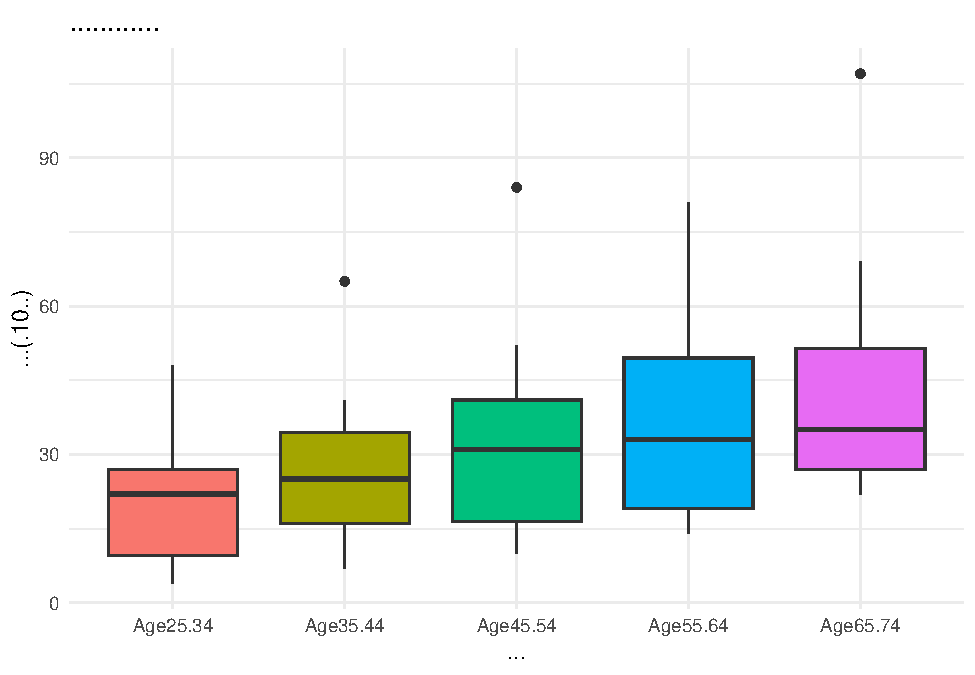
\includegraphics[keepaspectratio]{test_files/figure-latex/unnamed-chunk-17-1.pdf}}

从图中可以看出 年龄越大,自杀率整体水平越高,且数据波动越大。

65-74
岁组不仅中位数最高,离散程度也最大,需重点关注该年龄段的自杀预防干预;

25-34 岁组数据集中,自杀率相对稳定且偏低。

\subsection{7}\label{section-6}

\subsubsection{a}\label{a-5}

\begin{Shaded}
\begin{Highlighting}[]
\CommentTok{\#data(LaborSupply)}
\NormalTok{LaborSupply }\OtherTok{\textless{}{-}} \FunctionTok{read\_csv}\NormalTok{(}\StringTok{"LaborSupply.csv"}\NormalTok{)}
\end{Highlighting}
\end{Shaded}

\begin{verbatim}
## Rows: 5320 Columns: 7
## -- Column specification --------------------------------------------------------
## Delimiter: ","
## dbl (7): lnhr, lnwg, kids, age, disab, id, year
## 
## i Use `spec()` to retrieve the full column specification for this data.
## i Specify the column types or set `show_col_types = FALSE` to quiet this message.
\end{verbatim}

\begin{Shaded}
\begin{Highlighting}[]
\NormalTok{labor }\OtherTok{\textless{}{-}}\NormalTok{ LaborSupply }\SpecialCharTok{\%\textgreater{}\%} 
  \FunctionTok{mutate}\NormalTok{(}
    \AttributeTok{hour =} \FunctionTok{exp}\NormalTok{(lnhr),         }
    \AttributeTok{wage =} \FunctionTok{exp}\NormalTok{(lnwg),         }
    \AttributeTok{.before =}\NormalTok{ kids           }
\NormalTok{  ) }\SpecialCharTok{\%\textgreater{}\%} 
  \FunctionTok{select}\NormalTok{(}\SpecialCharTok{{-}}\NormalTok{lnhr, }\SpecialCharTok{{-}}\NormalTok{lnwg) }

\NormalTok{states }\OtherTok{\textless{}{-}}\NormalTok{ labor }\SpecialCharTok{\%\textgreater{}\%} 
  \FunctionTok{group\_by}\NormalTok{(year) }\SpecialCharTok{\%\textgreater{}\%} 
  \FunctionTok{summarise}\NormalTok{(}
    \AttributeTok{avg\_hours =} \FunctionTok{mean}\NormalTok{(hour),}
    \AttributeTok{sd\_hours =} \FunctionTok{sd}\NormalTok{(hour),}
    \AttributeTok{n =} \FunctionTok{n}\NormalTok{()}
\NormalTok{  )}

\CommentTok{\# 输出结果}
\NormalTok{states}
\end{Highlighting}
\end{Shaded}

\begin{verbatim}
## # A tibble: 10 x 4
##     year avg_hours sd_hours     n
##    <dbl>     <dbl>    <dbl> <int>
##  1  1979     2202.     502.   532
##  2  1980     2182.     454.   532
##  3  1981     2185.     460.   532
##  4  1982     2145.     442.   532
##  5  1983     2124.     550.   532
##  6  1984     2149.     492.   532
##  7  1985     2203.     515.   532
##  8  1986     2195.     482.   532
##  9  1987     2219.     529.   532
## 10  1988     2222.     478.   532
\end{verbatim}

\subsubsection{b}\label{b-5}

\begin{Shaded}
\begin{Highlighting}[]
\NormalTok{age\_hours\_1982 }\OtherTok{\textless{}{-}}\NormalTok{ labor }\SpecialCharTok{\%\textgreater{}\%}
  \FunctionTok{filter}\NormalTok{(year }\SpecialCharTok{==} \DecValTok{1982}\NormalTok{) }\SpecialCharTok{\%\textgreater{}\%}
  \FunctionTok{group\_by}\NormalTok{(age) }\SpecialCharTok{\%\textgreater{}\%}
  \FunctionTok{summarise}\NormalTok{(}\AttributeTok{avg\_hours =} \FunctionTok{mean}\NormalTok{(hour, }\AttributeTok{na.rm =} \ConstantTok{TRUE}\NormalTok{)) }\SpecialCharTok{\%\textgreater{}\%}
  \FunctionTok{arrange}\NormalTok{(}\FunctionTok{desc}\NormalTok{(avg\_hours))}


\NormalTok{max\_age\_group }\OtherTok{\textless{}{-}}\NormalTok{ age\_hours\_1982}\SpecialCharTok{$}\NormalTok{age[}\DecValTok{1}\NormalTok{]}

\FunctionTok{cat}\NormalTok{(}\StringTok{"1982年工作时长最长的年龄组为"}\NormalTok{, max\_age\_group, }\StringTok{"岁,平均工作时长为"}\NormalTok{, }
    \FunctionTok{round}\NormalTok{(age\_hours\_1982}\SpecialCharTok{$}\NormalTok{avg\_hours[}\DecValTok{1}\NormalTok{], }\DecValTok{2}\NormalTok{), }\StringTok{"小时"}\NormalTok{)}
\end{Highlighting}
\end{Shaded}

\begin{verbatim}
## 1982年工作时长最长的年龄组为 46 岁,平均工作时长为 2373.46 小时
\end{verbatim}

\subsubsection{c}\label{c-2}

\begin{Shaded}
\begin{Highlighting}[]
\NormalTok{id\_years }\OtherTok{\textless{}{-}}\NormalTok{ labor }\SpecialCharTok{\%\textgreater{}\%}
  \FunctionTok{group\_by}\NormalTok{(id) }\SpecialCharTok{\%\textgreater{}\%}
  \FunctionTok{summarise}\NormalTok{(}
    \AttributeTok{n\_years =} \FunctionTok{n\_distinct}\NormalTok{(year),      }
    \AttributeTok{first\_year =} \FunctionTok{min}\NormalTok{(year),          }
    \AttributeTok{last\_year =} \FunctionTok{max}\NormalTok{(year)           }
\NormalTok{  )}


\NormalTok{is\_balanced }\OtherTok{\textless{}{-}}\NormalTok{ (}\FunctionTok{length}\NormalTok{(}\FunctionTok{unique}\NormalTok{(id\_years}\SpecialCharTok{$}\NormalTok{n\_years)) }\SpecialCharTok{==} \DecValTok{1}\NormalTok{)}

\NormalTok{labor }\OtherTok{\textless{}{-}}\NormalTok{ labor }\SpecialCharTok{\%\textgreater{}\%}
  \FunctionTok{left\_join}\NormalTok{(id\_years[, }\FunctionTok{c}\NormalTok{(}\StringTok{"id"}\NormalTok{, }\StringTok{"n\_years"}\NormalTok{)], }\AttributeTok{by =} \StringTok{"id"}\NormalTok{)}

\FunctionTok{cat}\NormalTok{(}\StringTok{"面板数据平衡性判断:"}\NormalTok{, }\FunctionTok{ifelse}\NormalTok{(is\_balanced, }\StringTok{"平衡"}\NormalTok{, }\StringTok{"不平衡"}\NormalTok{))}
\end{Highlighting}
\end{Shaded}

\begin{verbatim}
## 面板数据平衡性判断: 平衡
\end{verbatim}

\subsubsection{d}\label{d-2}

\begin{Shaded}
\begin{Highlighting}[]
\NormalTok{id\_no\_kids }\OtherTok{\textless{}{-}}\NormalTok{ labor }\SpecialCharTok{\%\textgreater{}\%}
  \FunctionTok{group\_by}\NormalTok{(id) }\SpecialCharTok{\%\textgreater{}\%}
  \FunctionTok{summarise}\NormalTok{(}
    \AttributeTok{no\_kids =} \FunctionTok{as.integer}\NormalTok{(}\FunctionTok{all}\NormalTok{(kids }\SpecialCharTok{==} \DecValTok{0}\NormalTok{))  }\CommentTok{\# 1=全程无子女,0=有子女}
\NormalTok{  )}


\NormalTok{labor }\OtherTok{\textless{}{-}}\NormalTok{ labor }\SpecialCharTok{\%\textgreater{}\%}
  \FunctionTok{left\_join}\NormalTok{(id\_no\_kids, }\AttributeTok{by =} \StringTok{"id"}\NormalTok{)}

\NormalTok{prop\_no\_kids }\OtherTok{\textless{}{-}} \FunctionTok{mean}\NormalTok{(id\_no\_kids}\SpecialCharTok{$}\NormalTok{no\_kids)}
\FunctionTok{cat}\NormalTok{(}\StringTok{"全程无子女的个体占比:"}\NormalTok{, }\FunctionTok{round}\NormalTok{(prop\_no\_kids }\SpecialCharTok{*} \DecValTok{100}\NormalTok{, }\DecValTok{2}\NormalTok{), }\StringTok{"\%"}\NormalTok{)}
\end{Highlighting}
\end{Shaded}

\begin{verbatim}
## 全程无子女的个体占比: 8.08 %
\end{verbatim}

\subsubsection{e}\label{e-1}

\begin{Shaded}
\begin{Highlighting}[]
\NormalTok{wage\_compare\_1980 }\OtherTok{\textless{}{-}}\NormalTok{ labor }\SpecialCharTok{\%\textgreater{}\%}
  \FunctionTok{filter}\NormalTok{(year }\SpecialCharTok{==} \DecValTok{1980}\NormalTok{) }\SpecialCharTok{\%\textgreater{}\%}
  \FunctionTok{group\_by}\NormalTok{(no\_kids) }\SpecialCharTok{\%\textgreater{}\%}
  \FunctionTok{summarise}\NormalTok{(}
    \AttributeTok{avg\_wage =} \FunctionTok{mean}\NormalTok{(wage, }\AttributeTok{na.rm =} \ConstantTok{TRUE}\NormalTok{),   }
    \AttributeTok{sd\_wage =} \FunctionTok{sd}\NormalTok{(wage, }\AttributeTok{na.rm =} \ConstantTok{TRUE}\NormalTok{),      }
    \AttributeTok{count =} \FunctionTok{n}\NormalTok{()                            }
\NormalTok{  )}


\NormalTok{wage\_compare\_1980}
\end{Highlighting}
\end{Shaded}

\begin{verbatim}
## # A tibble: 2 x 4
##   no_kids avg_wage sd_wage count
##     <int>    <dbl>   <dbl> <int>
## 1       0     14.5    6.69   489
## 2       1     15.9    6.71    43
\end{verbatim}

\end{document}
